\section{Head Up Display (HUD)}
The HUD is turned on when switching the main mode selector
(\figref{fig:left-panel}{item:main-mode}) from~BER/PRE to~NAV.
It is powered by the secondary AC bus, and requires 30 seconds with AC power available before starting.

\subsection{Overview}
\begin{figure}[!ht]
  \centering
  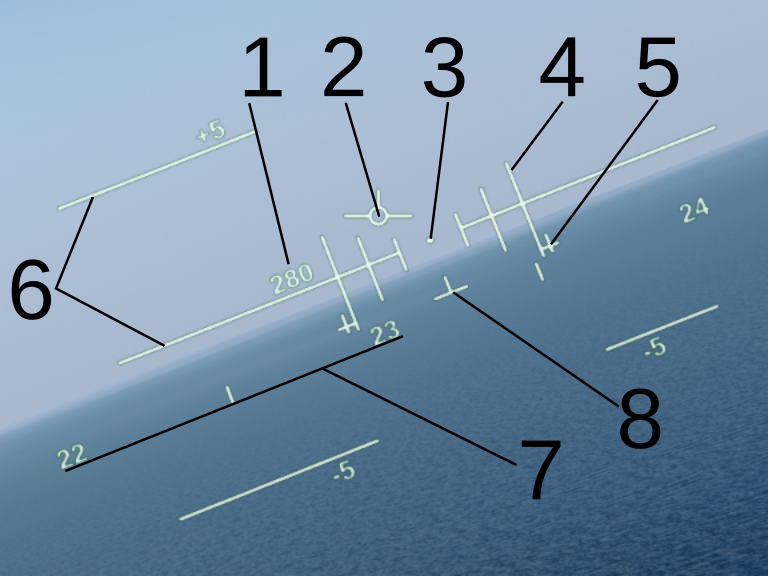
\includegraphics[width=0.6\textwidth]{images/displays/ajs-hud-general.png}

  \begin{multicols}{2}
    \begin{enumerate}[nosep]
      \item \label{item:digalt} Digital altitude
      \item \label{item:fpv} Flight path vector
      \item \label{item:refpt} Reference point
      \item \label{item:alt} Altitude bars
      \item \label{item:refbars} Reference bars and radar altitude index
      \item \label{item:horizon} Artificial horizon and pitch lines
      \item \label{item:heading-hud} Heading scale
      \item \label{item:timeline} Time / distance scale
    \end{enumerate}
  \end{multicols}

  \caption{HUD overview}
  \label{fig:hud}
\end{figure}

\subsection{Controls}
HUD brightness is adjusted with knob \figref{fig:front-panel}{item:hud-bright}.

The following two switches located on the lower right of the HUD
(\figref{fig:front-panel}{item:hud-switch}) affect the HUD presentation.

\paragraph{SLAV SI (SLV HUD)}
\label{sec:hud-slav-switch}
In navigation mode, this switch enables a decluttered low-altitude mode when
in position T (ON), see \cref{sec:hud-declutter}.

During optical landing, when in position T (ON), the HUD reference point will
be aligned with the flight path vector, instead of indicating runway heading.

\paragraph{HÖJD CI SI (ALT DISP)}
\label{sec:hud-alt-switch}
When in position RHM (RAD), the radar altimeter is used to compute a ground
corrected altitude, which is displayed on the HUD.
Otherwise, displayed altitude is the same as on the main altimeter.

The switch automatically goes back to position LD (BAR) at altitude >2450m
and during landing final phase.

\subsection{Navigation Mode}
\label{sec:hud-nav}
\paragraph{Artificial Horizon (\figref{fig:hud}{item:horizon})}
The artificial horizon and the $\pm 5 \degree$ pitch lines provide an attitude reference.
The HUD does not have a full pitch scale, only the horizon and the $\pm 5 \degree$ lines.

Horizontally, the artificial horizon is pointing towards the current destination,
indicated by the reference point (\figref{fig:hud}{item:refpt}).

\paragraph{Flight Path Vector (\figref{fig:hud}{item:fpv})}
The FPV marker indicates the aircraft path direction relative to the ground.
When on the horizon, the aircraft is in level flight.
When covering the reference point, the aircraft track coincides with the destination.

\paragraph{Digital Altitude (\figref{fig:hud}{item:digalt})}
Displays the aircraft altitude.
Below 1km the altitude is displayed in meters with a precision of 10m.
Above 1km the altitude is displayed in kilometers with a precision of 100m.
Above 10km, the digital altitude cycles back to 0,
thus 1500m and 11500m are both displayed as `1,5'.
Negative altitude down to -90m can be displayed.

\paragraph{Altitude Bars (\figref{fig:hud}{item:alt})}
The 6 altitude bars indicate the aircraft altitude relative to the reference altitude
(also called commanded altitude).

The top of the bars represents the reference altitude,
and the bottom of the bars represent ground level (to be exact, indicated altitude 0m).
The aircraft altitude is indicated by the horizon line.
Thus, if the top of the bars is aligned with the horizon, the aircraft is at the commanded altitude,
and if the bottom of the bars is aligned with the horizon, the aircraft is at ground level.

One can imagine the top, resp.\ bottom of the bars as forming a horizontal
plane in a perspective drawing, located at reference altitude, resp.\ ground altitude.
In this perspective drawing, the vanishing point is the reference point.

If the reference altitude is higher than 500m,
the bottom of the bars represents the reference altitude minus 500m instead of ground level.

\subparagraph{Reference Altitude}
\label{sec:ref-alt}
The reference altitude displayed by the altitude bars is set as follows.
\begin{itemize}[noitemsep]
  \item During takeoff, reference altitude is fixed at 500m.
  \item During flight, the reference button (keybinding \keys{\shift+R}) 
    sets it to the current altitude.
  \item If autopilot altitude hold mode is active,
    the reference altitude is the autopilot altitude.
  \item When entering landing mode, reference altitude is set to 500m.
    It can still be modified with the reference button or by engaging autopilot altitude hold.
\end{itemize}

If the difference between reference altitude and current altitude is too large,
the displayed reference altitude will differ from the actual reference altitude.

\subparagraph{Reference Altitude Bars (\figref{fig:hud}{item:refbars})}
The reference altitude bars are located just next to the outer altitude bars.
The length of the reference altitude bars varies to indicate reference altitude:
if the length of the outer altitude bars (which is fixed to 3\textdegree{})
represents the reference altitude, then the length of the reference altitude bars represents 100m.

For instance, in \cref{fig:hud}, the length of the reference altitude bars is
0.6\textdegree{}, i.e.\ 1/5 of the outer altitude bars.
Thus 100m is 1/5 of the reference altitude, i.e.\ the reference altitude is 500m.

At reference altitudes higher than 500m, the reference bars are hidden.

\subparagraph{Radar Altitude Index (\figref{fig:hud}{item:refbars})}
When available, radar altitude is indicated by a horizontal index on the outer altitude bars,
which can be read on the outer altitude bars or the reference altitude bars.

When the index is at the bottom of the altitude bars,
radar altitude and indicated altitude coincide,
which can be used to calibrate the altimeter in flight.
However this method is only accurate when reference altitude is at most 500m
(reference altitude bars are displayed).

\paragraph{Heading Scale (\figref{fig:hud}{item:heading-hud})}
Indicates current heading.
Every 10\textdegree{} is indicated by a number,
and every 5\textdegree{} between them by a vertical mark.
The scale is 1:1, i.e.\ the bearing of a world object can be read directly on the scale.

\paragraph{Time and Distance Scale (\figref{fig:hud}{item:timeline})}
Indicate time or distance to an event or waypoint.
The line shrinks and grows horizontally around the center to indicate time or distance to the event.
A vertical center mark, and in some modes two side marks, represent the events.
\begin{itemize}
  \item During takeoff roll, the line grows to indicate aircraft speed.
    The side marks indicate recommended rotation speed.
  \item In navigation mode, the line represents time to the next waypoint.
    It appears 60 seconds before the waypoint, and shrinks until reaching the waypoint.
  \item In aiming modes, the line represents distance to the target. See \cref{chap:weapons} for details.
\end{itemize}

\subsection{Low Altitude Declutter}
\label{sec:hud-declutter}
If the switch SLAV SI is in position T (TILL), a decluttered HUD is displayed at altitude <100m.
In this decluttered mode, only the flight path vector,
artificial horizon, and digital altitude are displayed.
Pressing the reference button (keybinding \keys{\shift+R})
in decluttered mode toggles the heading scale.

\subsection{Takeoff Mode}
Takeoff mode is enabled is enabled when the nose gear is compressed,
provided the master mode selector is not in mode LANDING.

During takeoff, the FPV is fixed 10\textdegree{} below the aircraft forward axis,
and the FPV marker vertical fin is hidden.
The artificial horizon reference point is aligned with the aircraft forward axis.
Time line and heading scale are fixed 10\textdegree{} below the horizon.
The time line indicates airspeed, with the side markers corresponding to rotation speed.

When the rotation angle reaches 5\textdegree{},
the time line is hidden and the heading scale moves to its normal position.
Takeoff mode stops once the airspeed exceeds M 0.35,
when the climb angle is at least 3\textdegree{},
or at landing gear retraction.

\subsection{Landing Mode}
\begin{figure}[!ht]
  \centering
  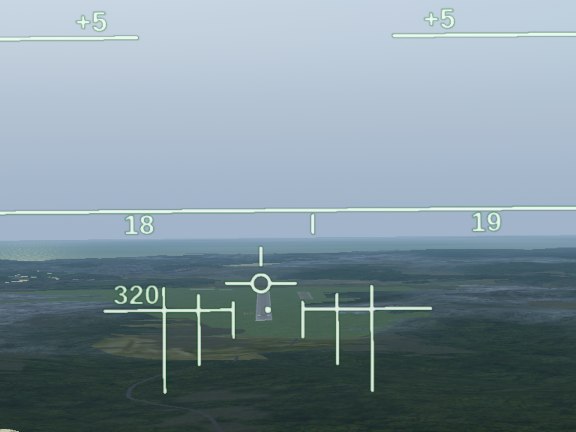
\includegraphics[width=0.5\textwidth]{images/displays/ajs-hud-landing.png}
  \caption{HUD during final}
  \label{fig:hud-landing}
\end{figure}

In landing mode, the HUD changes when starting the final.
The -5\textdegree{} pitch lines are removed,
and a glideslope line is added 2.86\textdegree{} below the horizon
(corresponding to a slope of 5\%).
Altitude bars and digital altitude are moved from the horizon to the glideslope line,
and the heading scale is moved under the horizon.

\paragraph{Speed / AoA Indicator}
In landing mode, the vertical fin (`tail') of the flight path vector symbol
moves vertically to indicate deviation from the target speed or angle of attack.
The speed is correct when the bottom of the tail is on the FPV circle
(default position in navigation mode).
If the tail is higher than the circle, the aircraft speed is too high.
If the tail is lower (inside the circle), the aircraft speed is too low.

While the landing gear is up, the target speed is 550km/h.
Once the landing gear is down and locked, the target angle of attack is 12\textdegree{}.
If the $\alpha 15,5\degree$ button
(\figref{fig:front-panel}{item:autothrottle-lights}) is pressed (light lit),
the target angle of attack is 15.5\textdegree{} instead.

When the landing gear is down, the fin will blink if the angle of attack is critically high.

\paragraph{ILS Guidance}
If ILS guidance is used, the reference point indicates the heading to follow to align with the localizer,
and the altitude bars indicate ILS glideslope deviation:
if the top of the bars is above, resp.\ below the glideslope line,
the aircraft is below, resp.\ above the ILS glideslope.

If ILS is not used (optical landing mode),
the reference point indicates runway heading and the altitude bars are hidden.

\paragraph{Touchdown}
Below 30m, the HUD switches to optical landing display (ILS indications disappear).
Below 15m radar altitude, the HUD switches to flare mode.
The glideslope line moves up to indicate the descent angle
which gives a vertical speed of 2.96m/s, the maximum for touchdown.
If radar altitude is unavailable, transition to flare mode occurs at 30m.

\subsection{Tactical Information}
Some weapons have specific combat HUD presentations (aiming mode),
enabled by switching to ANF/CBT mode or arming the weapon.
See \cref{chap:weapons} for details.


\section{Radar Display (CI)}
The PS-37/A radar mounted on the AJS-37 is an X-band monopulse non-doppler radar.
It is designed as navigation aid, and to detect ships---and to some extent aircrafts.
It is somewhat similar to the radars commonly found on ships for navigation and collision avoidance.
The radar picture is displayed with only relatively basic filters applied:
interpreting it is up to the pilot.
In particular, the radar is not capable of locking or tracking targets.

\begin{figure}[!ht]
  \centering
  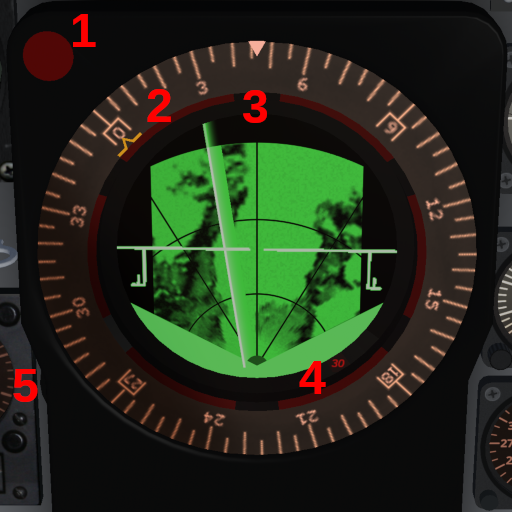
\includegraphics[width=0.6\textwidth]{images/displays/CI-overview.png}

  \begin{enumerate}[nosep]
    \item \label{item:alt-warning} Altitude warning light
    \item \label{item:heading-CI} Heading indicator (see \cref{sec:flight-instruments})
    \item \label{item:rwr-lights} Radar Warning Receiver (6 lights in a ring)
    \item \label{item:radar-range} Radar range indicator, in km
    \item \label{item:CI-polaroid-filter} CI polarizing filter (adjusts brightness and color of display)
  \end{enumerate}

  \caption{Overview of the CI display}
  \label{fig:CI}
\end{figure}

\subsection{Display}

\paragraph{Radar Picture}
The CI radar display is a Plan Projection Indicator (PPI),
showing an undistorted map of the terrain in front of the aircraft.
The aircraft position is represented by the bottom corner.
The radar sector spans 61.5\textdegree{} on either side of the center line,
and extends to up to 120km, depending on the radar range.
Dark parts of the radar picture correspond to strong radar echoes.

\paragraph{Radar Symbols}
The following reference lines are displayed in black on the radar picture.
\begin{itemize}
  \item Three azimuth reference lines, straight ahead and 30\textdegree{} on either sides.
  \item Up to four distance reference arcs, at 10km, 20km, 40km, and 80km.
    These distances remain the same regardless of the radar range:
    when radar range is 15km only the 10km arc will be visible,
    while when radar range is 120km all four arcs are visible.
\end{itemize}

\paragraph{Navigation Symbols}
The following bright navigation symbols are overlayed on the radar picture.
\begin{itemize}
  \item Whenever a waypoint is selected as destination,
    it is displayed as a circle (\cref{fig:CI-navigation-waypoint}).
  \item In addition, when the selected waypoint is the departure or arrival airbase,
    a 20km long line representing the approach path for the selected runway is added
    (\cref{fig:CI-navigation-runway}).
  \item In landing mode, during the initial approach phase, a circle with radius 4.1km
    is displayed tangent to the approach line, at the end opposite of the runway (\cref{fig:CI-navigation-landing}).
    The aircraft should fly along the border of this circle until it is aligned with the approach line.
\end{itemize}

\begin{figure}[!ht]
  \centering
  \begin{subfigure}[t]{0.3\textwidth}
    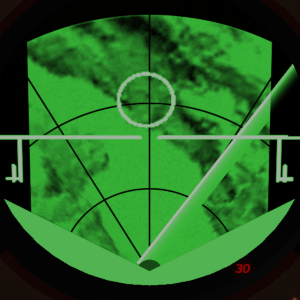
\includegraphics[width=\textwidth]{images/displays/CI-waypoint.png}
    \caption{Waypoint circle}
    \label{fig:CI-navigation-waypoint}
  \end{subfigure}
  \begin{subfigure}[t]{0.3\textwidth}
    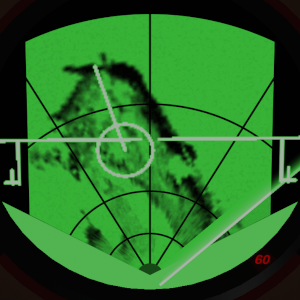
\includegraphics[width=\textwidth]{images/displays/CI-runway.png}
    \caption{Approach line}
    \label{fig:CI-navigation-runway}
  \end{subfigure}
  \begin{subfigure}[t]{0.3\textwidth}
    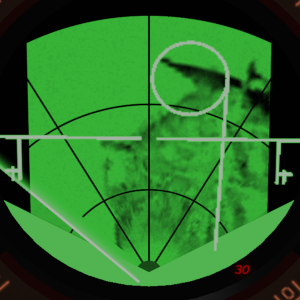
\includegraphics[width=\textwidth]{images/displays/CI-landing.png}
    \caption{Landing mode}
    \label{fig:CI-navigation-landing}
  \end{subfigure}

  \caption{CI navigation symbols}
  \label{fig:CI-navigation}
\end{figure}

\paragraph{Artificial Horizon}
An artificial horizon is displayed across the CI with bright symbols.
It consists of a fixed reference mark (two short horizontal lines in the center) representing the flight path vector,
the horizon itself moving around this mark,
as well as altitude bars, altitude reference bars, and radar altimeter indices.
These display the same information as the HUD, see \cref{sec:hud-nav}.


\subsection{Radar and CI Operation}

\paragraph{Power}
The CI is powered by the secondary AC bus.
After switching from mode BER/PRE to NAV with AC power available,
the CI begins a 30 seconds startup and preheating sequence.
After this, the CI is turned on/off with \keys{R}/\keys{F}.
In landing modes, or when passive reconnaissance is selected on the radar panel,
The CI will also always remain on.

The radar itself is also turned on/off with \keys{R}/\keys{F},
when the following conditions are met:
\begin{itemize}[nosep]
  \item Secondary bus AC, secondary bus DC, and hydraulic power are available.
  \item Power has been available for 3 minutes, for the radar to complete startup and pre-heating.
  \item Nose landing gear is uncompressed.
  \item Main mode selector (\figref{fig:left-panel}{item:main-mode}) is not in mode~BER/PRE or~FK/TST.
\end{itemize}

\paragraph{Radar Modes}
The following radar modes are obtained with main mode selector in position NAV, SPA/REC, or LANDING.
\begin{description}
  \item[Normal mode]
    This is the radar mode obtained when starting the radar.
    The radar scans a sector of 61.5\textdegree{} on either side, at a rate of $110\degree{}/s$.
    The radar antenna is tilted between $0.5\degree{}$ and $3\degree{}$ down
    depending on altitude and radar range.
    This angle is convenient to scan the terrain at altitudes of a few hundred meters.

    To return to normal mode, turn the radar off and on again.
  \item[Memory mode]
    Obtained by pressing \keys{\shift+F} in normal mode.
    The radar turns off, and the CI continues to show the last radar image.
    This image will slowly decay, it remains readable for at least 30 seconds.
  \item[Terrain mode]
    Obtained by pressing \keys{\ctrl+F} in normal or memory mode.
    Similar to normal mode except (1) the radar antenna tilt angle is 0\textdegree{},
    and (2) the radar beam is narrower in height.
    This strongly highlights any terrain at the same altitude as the aircraft,
    thus helping to avoid collision with terrain in low level flight.
\end{description}

When the main mode selector is in position ANF/CBT, the radar mode depends on the selected weapon:
\begin{description}
  \item[Rb 04, Rb 15, m/90] Similar to normal mode.
    The CI center line rotates slightly to indicate the aircraft ground track, thus helping with aiming.
    For the Rb 04 only, two short arcs are added to the center line, indicating minimum and maximum firing range.
    The memory submode is available, but not the terrain submode.
  \item[A/A mode] (Sidewinders, AKAN or Rb 05 in A/A mode)
    Similar to normal mode, but the radar antenna is tilted 1.5\textdegree{} up,
    and the radar beam is narrower in height.
    Memory and terrain submodes are unavailable.
  \item[A/A ranging mode] In A/A mode, press \keys{L} to enter A/A ranging mode.
    The radar antenna is aligned with the HUD aiming reticle,
    and measures range to an aircraft behind this reticle (if any).
    The range is displayed by the distance line on the HUD.
    The CI is off in this mode. Turn the radar off and on again to return to A/A mode.
  \item[A/G ranging mode] (AKAN, ARAK, bombs, Rb 05, Rb 75)
    CI turns off. Depending on the weapon and aircraft attitude,
    the radar may be used to measure distance to ground, which is displayed by the HUD distance line.
\end{description}

\paragraph{Antenna angle}
The radar antenna default tilt angle is determined by the radar mode, see above.
This tilt angle can be adjusted $\pm 10 \degree$ from the default position with \keys{<}/\keys{>}.
A `click' is heard when returning to the default position.
In A/A mode only, an antenna tilt angle indicator is displayed at the top of the CI.
It consists of a mark moving along an horizontal line (left is down, right is up).

\paragraph{Radar gain}
The radar gain (strength of displayed radar echoes) can be adjusted with \keys{\{}/\keys{\}}.
The default setting is appropriate for sea navigation, with all coastline giving fairly strong returns.
Over land, it is usually convenient to lower the radar gain
to get better contrast between different types of terrain.
A `click' is heard when returning to the default gain position.


\subsection{Interpreting Radar Pictures}
To understand what is displayed by the radar,
it is useful to know how different types of terrain reflect radar waves.
\begin{description}
  \item[Water] forms a relatively smooth surface, which tends to reflect radar waves \emph{away} from the aircraft.
    Thus water gives very little radar returns, and shows as bright areas.
    Strong waves may make it more noisy.

  \item[Land] is more irregular, and tends to diffuse radar waves in all direction,
    thus giving stronger radar returns than water.
    They appear in intermediate tones, varying with relief and terrain type.

  \item[Hills] facing the aircraft have a significant area which can
    reflect or diffuse radar waves towards the aircraft, thus giving very strong radar returns.
    Furthermore, the area behind the hills is obstructed, and gives no radar returns.
    Thus close side of hills appears as a very dark band, followed by an empty area for the obstructed side.

  \item[Urban areas] tend to give strong radar returns because buildings
    can reflect radar waves towards the aircraft, and even act as corner reflector.
    They appear as dark and noisy areas.
\end{description}
See \cref{fig:CI-radar} for an example of such terrain types:
\begin{enumerate}[nosep]
  \item The bright area in the middle is a lake.
  \item Immediately to the right of the lake is some relatively flat land, in mid tones.
  \item Further is a large ridgeline, appearing as a black band.
    Terrain beyond this ridge is not visible, the corresponding area of the CI is empty.
  \item On the left is a more irregular terrain, which shows as a mix
    of dark patches (hills facing the aircraft) and empty zones (hidden terrain).
\end{enumerate}

\begin{figure}[!ht]
  \centering
  \begin{subfigure}[t]{0.49\textwidth}
    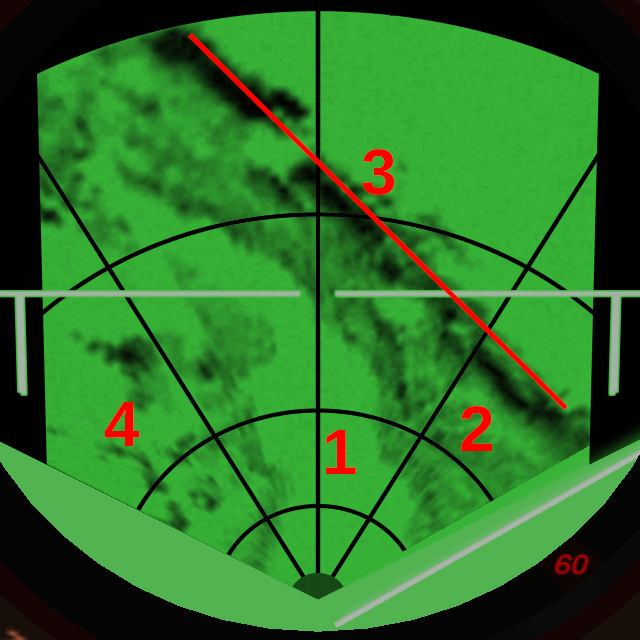
\includegraphics[width=\textwidth]{images/displays/CI-radar.png}
    \caption{Radar picture.}
  \end{subfigure}
  \begin{subfigure}[t]{0.49\textwidth}
    \includegraphics[width=\textwidth]{images/displays/léman_map_stamen.png}
    \caption{Map of the same area.}

    {\centering \footnotesize Map tiles by Stamen Design, data by OpenStreetMap.}
  \end{subfigure}

  \caption{%
    Example of radar picture over Lac Léman with easily identifiable terrain features.
  }
  \label{fig:CI-radar}
\end{figure}
